La oferta de tecnologías a la hora de realizar un proyecto software es realmente extensa. A menudo la elección de estas tecnologías para formar la pila de desarrollo está vagamente justificada y el mayor argumento suele ser la familiaridad de los desarrolladores con las herramientas escogidas. Esto, de hecho, no es un argumento menor, ya que en un entorno real, adquirir los conocimientos suficientes sobre una serie de tecnologías como para crear un producto listo para la explotación necesita una gran cantidad de tiempo por parte del equipo de desarrollo y por ende también supone un importante costo económico. Sin embargo, sí que deberían conocerse los puntos débiles y fuertes de las principales opciones y debería realizarse un análisis para evitar problemas graves en el futuro. En este capítulo se describen las tecnologías empleadas para la realización de este proyecto y la justificación de la elección realizada. No se listan dependencias triviales, y que tengan un propósito inmediato (leer ficheros, crear archivos temporales, etcétera).


\section{GitHub}
GitHub es el eje central de todo este trabajo. A pesar de que no sea una plataforma enfocada en la enseñanza, es innegable el valor y productividad que proporcionada a virtualmente todos los desarrolladores de software del mundo. Los profesores pueden gestionar las clases en el mismo ámbito en el que se desarrollan las prácticas o tareas, y con la herramienta desarrollada en este trabajo pretendemos reducir el cambio de contexto y redundancia que sufren los alumnos entre el Moodle de la institución (o cualquier programa de la misma índole) y GitHub.

\subsection{GitHub CLI} 
Como se ha comentado anteriormente, Github CLI\cite{gh-cli} y su comando \verb|gh extension| nos permite crear programas destinados a la interacción con GitHub y es la base sobre el cual se construye este proyecto, permitiéndome a mí como programador y diseñador crear un código sostenible, aprovechar comandos comunes creados por el equipo de GitHub y aumentar las posibilidades de integrarme con otros programas creados por otros miembros de la comunidad.

Quiero mencionar los comandos \verb|gh api|\cite{gh-api} y \verb|gh auth login|\cite{gh-auth-login}. El primero sirve para realizar peticiones HTTP (\verb|API REST| y \verb|GraphQL|) imprimiendo la respuesta, y el segundo autentifica al usuario con un token y guarda información del usuario. Son especialmente útiles porque no tengo que pedir constantemente los credenciales y demás datos del usuario, por lo que no solo las peticiones son más sencillas, sino que me ayuda bastante en hacer que la aplicación sea segura.

\subsection{Las APIs de GitHub: REST y  GraphQL}
Las \verb|API|s que nos proporciona GitHub son completamente necesarias. Sin ellas no podríamos tener ningún tipo de comunicación con los servicios de GitHub.

Se proveen dos APIs: \verb|API REST|\cite{github-rest-api} y GraphQL\cite{github-graphql}. En este trabajo se hace uso de las dos, pero la \verb|API REST| queda relegada para casos sencillos. Se ha decidido de esta forma, pues con \verb|GraphQL| podemos obtener solo los datos que queremos, y podemos recibir en una única llamada información que de otra forma requeriría varías llamadas a diferentes \emph{endpoints}.

\section{El buscador difuso fzf}
La aplicación \verb|fzf| \cite{fzf} del inglés \emph{fuzzy finder} es un \href{https://en.wikipedia.org/wiki/Approximate_string_matching}{buscador difuso} para la línea de comandos.
Nos permite de manera interactiva filtrar de cualquier lista uno o varios elementos de una forma muy rápida.
Su uso es muy minimalista y simple: el programa lee de la \verb|STDIN| (estándar input) y los elementos seleccionas son escritos a la \verb|STDOUT| (estándar output)
Entre sus características, las que se han usado en este proyecto son:
\begin{itemize}
    \item Previsualización del elemento seleccionado \ref{fig:interface-log}
    \item STDIN dinámico
    \item Selección múltiple \ref{fig:clone}
    \item Personalización de la interfaz \ref{fig:clone} \ref{fig:interface-log}
\end{itemize}
El usuario también puede hacer uso de su \href{https://github.com/junegunn/fzf#search-syntax}{sintaxis de búsqueda} para agilizar el filtrado de elementos

Uno de los problemas principales a la hora de usar \verb|fzf| es que no es una librería, sino un programa independiente distribuido como un binario. Esto significa que se tiene que invocar como un comando externo, y en el caso de \verb|shelljs|, características como el STDIN dinámico son difíciles de usar. Aparte le tenemos que pedir al usuario que tenga instalado \verb|fzf| y este disponible en el \verb|PATH|.

Otro punto más preocupante es que \verb|fzf| utiliza \verb|STDERR| para mostrar la interfaz, probablemente debido a que la \verb|STDOUT| ya está siendo utilizada para devolver la selección del usuario, es decir, el resultado al presionar \emph{ENTER}. Esto significa que los errores están siendo escritos en un descriptor de archivos que ya está siendo utilizado. Para los errores propios de \verb|fzf| no hay ningún problema, pues la aplicación se cancela antes de mostrar ningún error, pero cuando se está ejecutando en conjunto con otros programas acaparar la \verb|STDERR| no es buena idea y puede generar comportamiento indefinido, dependiendo de como cada emulador de terminal maneje este tipo de situaciones.

\section{Los Lenguajes JavaScript y TypeScript (Node.js)}
El lenguaje de programación escogido es \verb|JavaScript|\cite{js} (a partir de ahora \verb|JS|) en su implementación de Node.js. Los motivos son variados. Por un lado, es uno de los lenguajes con el que tengo más experiencia y destreza programando. A su vez, si tenemos en cuenta que está en el top de lenguajes más usados \href{https://www.jetbrains.com/es-es/lp/devecosystem-2021/#Main_programming-languages}{en} \href{https://insights.stackoverflow.com/survey/2021#technology-most-popular-technologies}{varias} \href{https://www.tiobe.com/tiobe-index/}{listas}, es más fácil encontrar gente que esté dispuesta a contribuir al núcleo y sus principales extensiones. Así mismo, como es tan común, los usuarios no tendrían que estar instalando dependencias de más.

Dejando de lado su popularidad y centrándonos en propiedades más intrínsecas del lenguaje, podemos ver que no hay mejor lenguaje para el manejo de ficheros JSON (usado por las API de GitHub), también al ser un lenguaje interpretado y flexible me ha permitido ser muy productivo en la fase de diseño y prototipado.

Pasada la fase de diseño y prototipado, se decidió reescribir el \verb|core| en TypeScript \cite{ts}, con el objetivo de minimizar bugs y aprovechar una mejor integración con editores de texto compatibles con: autocompletado inteligente, saltos a referencias, refactorización, etc. Debido a que dicho código ya estaba empezando a alcanzar un tamaño considerable.

Donde más beneficio ha resultado TypeScript,
ha sido en el control del archivo de datos, 
{\tt data.json} (véase Figura \ref{fig:data}).
Al ser el punto central donde se escriben y 
se leen los datos, varías partes del \verb|core| 
dependen que dicho fichero tenga una cierta estructura. 

Por ejemplo, 

\begin{itemize}
    \item el comando \verb|gh edu reset| tiene 
    que reescribir casi todos los campos a su estado por 
    defecto (o todos si se utiliza el flag \verb|--force|), 
    \item 
    \verb|gh edu update -c| necesita saber 
    en qué parte estamos guardando la \gls{cache}. 
    \item 
    Si cambio el nombre o añado nuevos campos, 
    TypeScript me avisa con errores de compilación de 
    que los comandos dependientes también tiene que cambiar y 
    adaptarse a la nueva estructura. 
\end{itemize}

Esto también es aplicable en menor medida a todos 
los puntos donde se utiliza un objeto \verb|JS|.

Un ejemplo de los beneficios de TypeScript se puede 
ver en el esquema mínimo de {\tt data.json} 
(Figura \ref{fig:configType})

\begin{figure}[htb]
    \centering
    \makebox[\textwidth][c]{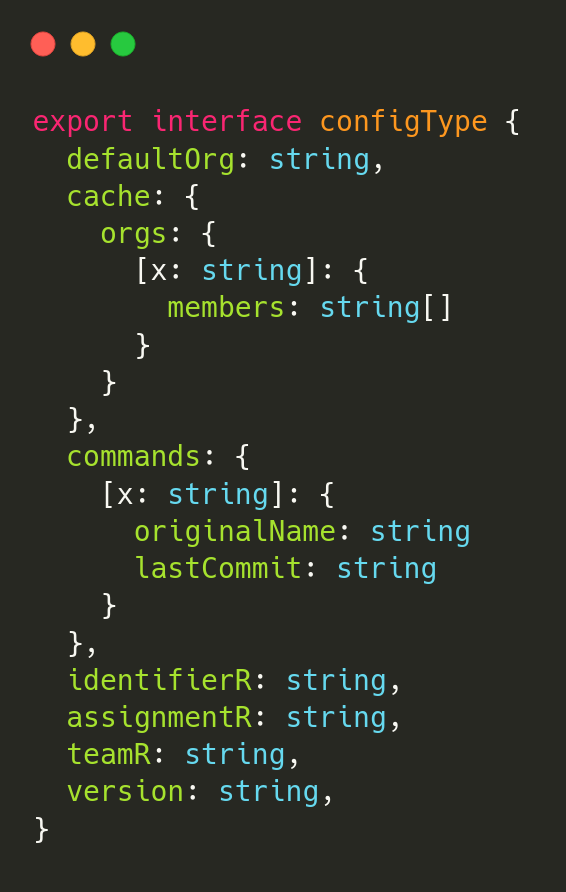
\includegraphics[width=0.5\textwidth]{images/configType.png}}
    \caption{Tipado fuerte en el archivo de datos}
    \label{fig:configType}
\end{figure}

No obstante, TypeScript es un lenguaje compilado y como tal requiere de su propio compilador. 
Esto añadiría otra dependencia al sistema aparte de Node.js. 
Más preocupante aún sería pedirle a nuestro usuario que compilase el código cada vez que vaya a instalar o actualizar.
Hay otras herramientas como \href{https://www.npmjs.com/package/ts-node}{ts-node} que nos permitirían ejecutar el código directamente, pero no solo estamos añadiendo más dependencias, sino que el tiempo de arranque de la aplicación se vería enormemente afectado, incluso si se utiliza un \gls{JIT}(\emph{just-in-time compiler}). 
Para solucionar estos problemas se ha optado por hacer compilación anticipada o \gls{AOT} (ahead-of-time) en cada \emph{commit} que se realice con un hook\cite{hook} de \verb|Git|.

%En el apartado de diseño[TODO añadir referencias] se explica en más detalle los efectos que ha tenido esta estrategia.

En cuanto a dependencia de desarrollo, se ha usado como gestor de paquetes \verb|npm|\cite{npm} por mera preferencia personal.

\subsection{La librería {\tt commander}}
La librería \verb|commander| es muy popular para la creación de aplicaciones \gls{CLI}, se encarga de parsear los argumentos y flags de la línea de comandos, de los mensajes de error relacionados con la creación de dichos argumentos e implementa un sistema de ayuda basándose en las especificaciones establecidas.

Es una parte esencial del ecosistema, a efectos prácticos genera la interfaz mínima necesaria, entre el usuario y el programa y la solución nativa \verb|process.argv| es muy pobre y primitiva en comparación.

Los motivos por los cuales se ha optado específicamente por \verb|commander| son:
\begin{itemize}
    \item \textbf{Popularidad.} Lo cual se traduce en un software a prueba de errores y con abundante documentación.
    \item \textbf{Cero dependencias.} Es bastante remarcable que un paquete del ecosistema de \verb|JS| sea autosuficiente, y nos ayuda en minimizar el tamaño y mantenimiento de nuestro software, en especial en la parte del \verb|core| que interesa que sea lo más convenientemente ligero.
\end{itemize}

\subsection{La librería {\tt shelljs}} \label{shelljs}
La librería {\tt shelljs} es el paquete que me permite llamar a comandos de la terminal desde el código fuente, independientemente del sistema operativo.

Incluye comandos propios de los sistemas Unix como \verb|cp|, \verb|rm| o \verb|which| entre otros, y un comando \verb|exec| para ejecutar cualquier otro comando no contemplado por su API.

Es bastante trivial de usar, pero su interfaz es algo pobre ante todas las posibilidades que ofrece la terminal. Alimentar la \verb|STDIN| con variables del programa, cuando el comando ya ha empezado su ejecución, o mandar una señal de cierre, no es posible al momento de escribir estas líneas. Ha habido intentos de ofrecer una \href{https://github.com/shelljs/shelljs/pull/432}{solución apropiada}, pero no ha habido avances, por lo que se ha tenido que recurrir a soluciones alternativas. Se puede ver una explicación más detallada y el porqué este comportamiento es necesario en el capítulo \textbf{Implementación}, en la sección de \verb|gh-edu-data| (\ref{impl:gh-edu-data}).

\subsection{La librería inquirer}
La librería \verb|inquirer| me permite conseguir datos del usuario de forma interactiva (figura \ref{fig:data-desiredData}). Es una colección de interfaces comunes como:
\begin{itemize}
    \item Confirmación
    \item Múltiple selección (checkbox)
    \item Listas a la \verb|fzf|
\end{itemize}

El método principal para conseguir input del usuario de forma interactiva es \verb|fzf|. La librería \verb|inquirer| carece de  características como la búsqueda difusa o \verb|stdin| dinámico. La utilidad \verb|fzf| es una herramienta diseñada para trabajar con listas.  En aquellas ocasiones que se requiere una simple confirmación o que el usuario tenga que escribir manualmente, se recurre a \verb|inquirer|. 

A pesar de no ser tan potente como \verb|fzf|, \verb|inquirer| es una librería nativa de \verb|JS|, por lo que ha sido más fácil trabajar con ella, especialmente en lo referente al manejo de errores.

\section{El Lenguaje Go} \label{go}
En una de las extensiones se utiliza el lenguaje de programación Go \cite{go}, el motivo de su uso se explica mejor en su respectivo apartado (\ref{diseño:gh-edu-plagiarism}).

Go es un lenguaje relativamente moderno (2009), que ha tenido una aceptación rápida en las tecnologías de la nube, como pueden ser servidores, pero también se ha utilizado mucho en el desarrollo de aplicación de terminal, de hecho, \verb|GitHub CLI| y su predecesor \verb|hub| han sido desarrollados usando Go.

Dentro del ámbito de este proyecto, las ventajas de Go son varias:
\begin{itemize}
    \item \textbf{Binario enlazado estáticamente.} Por lo que los usuarios no tiene que tener instalado \verb|Go|
    \item \textbf{Arranque inmediato.} A medida que las extensiones y el \verb|core| escritos en \verb|JS|/\verb|TypeScript| iban creciendo en tamaño y en dependencias de desarrollo, el rendimiento de la aplicación iba decayendo. Por lo general no es especialmente notorio ni grave, pero donde más se nota es cuando la aplicación empieza la ejecución, principalmente debido a los procesos que se tienen que ejecutar al inicio, como la validación del archivo de datos o la carga de extensiones instaladas.
    \item \textbf{Mejor integración con la terminal.} Los paquetes \href{https://pkg.go.dev/os}{os} e \href{https://pkg.go.dev/io}{io} de la librería estándar han sido de gran ayuda. He podido utilizar todas las características de \verb|fzf| y \verb|jq| manteniendo un código legible y mantenible.
    \item \textbf{Manejo de errores.} El manejo de errores en Go es bastante explícito. Esto hace que el código sea más verboso, pero tengo la seguridad de que mi aplicación tiene todos los posibles errores cubiertos. El usuario no va a ver ningún \emph{stack trace}, a no ser que el mensaje de error este destinado al programador.
\end{itemize}

En cuanto a desventajas, podemos hablar de la distribución:

\begin{itemize}
    \item Go es un lenguaje compilado: a diferencia de TypeScript, no compila a código fuente, sino a código máquina. 
    \item El propio equipo de \verb|gh| proporciona una GitHub Action \cite{githubAction} con nombre \href{https://github.com/cli/gh-extension-precompile}{gh-extension-precompile} que compila el código y lo guarda en el apartado de ``Releases`` de GitHub, a la hora de instalar o actualizar, el comando \verb|gh extension install| que se utiliza de forma interna, descarga el binario para el sistema operativo y arquitectura apropiados. 
    \item Esto ralentiza la productividad al tener que esperar que se compile a todas las plataformas (Linux, Mac OS, Windows) antes de poder probar los resultados con el resto del ecosistema.
\end{itemize}

\begin{figure}[htb]
    \centering
    \makebox[\textwidth][c]{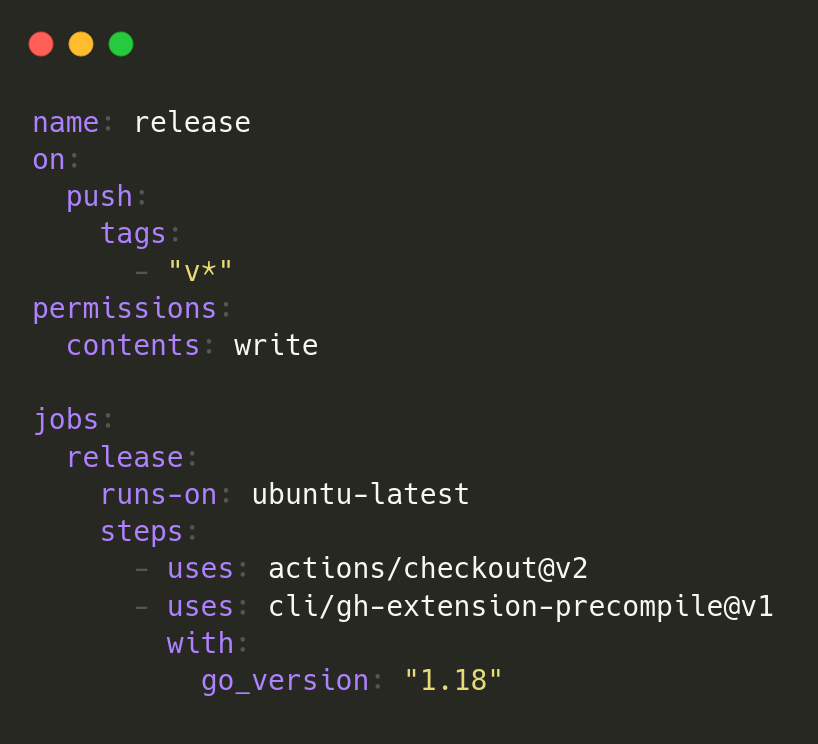
\includegraphics[width=0.5\textwidth]{images/gitHubRelease.png}}
    \caption{Script GitHub release}
    \label{fig:gitHubRelease}
\end{figure}

\subsection{La librería cobra}
La librería cobra \cite{cobra} es para \verb|Go| lo que commander es para javascript: Una librería que permite crear aplicaciones de líneas de comandos no triviales. Generando ayuda automáticamente, autocompletado y con una integración perfecta con viper.

\subsection{La librería viper}
La librerìa
{\tt viper}\cite{viper} es una librería para leer archivos de configuración, en este caso data.json. 
También me permite enlazar datos que se puedan conseguir desde variables de entornos, línea de comandos o archivo de configuración en una sola variable, en ese orden de prioridad.

\section{El Lenguaje jq (JSON Query)}

Para el manejo no trivial de ficheros \verb|JSON| se ha usado el \gls{DSL} jq\cite{jq}, un lenguaje de muy alto nivel que nos permite procesar ficheros \verb|JSON| desde la terminal. 

Si bien es cierto que uno de los motivos para usar \verb|JS| como lenguaje de desarrollo fue la facilidad con la que podemos manejar los ficheros \verb|JSON|, \verb|jq| puede ser más productivo cuando se trabaja en el contexto de la terminal, como es el caso cuando se trabaja con programas como \verb|gh api| o \verb"fzf", que  producen o procesan información en formato JSON a través de los canales o pipelines. 

Procesar JSON con \verb|jq| puede simplificar la tarea de previsualizar información adicional de un \emph{elemento} que está siendo seleccionado. Véase, por ejemplo, la extensión {\tt gh-edu-view} (\ref{sec:gh-edu-view-implementation}).

\section{El Lenguaje \LaTeX{} y Overleaf}
Para la elaboración de este documento se ha usado \LaTeX{}, 
en específico la implementación de \href{https://www.overleaf.com/}{overleaf}\cite{overlife}.
Gracias a esto hemos podido sincronizar con GitHub,
mantener un historial del documento, 
se ha simplificado la instalación de paquetes  y 
tenemos una copia accesible en línea que se sincroniza automáticamente
